\documentclass[twocolumn,11pt]{IEEEtran}
\usepackage[verbose,expansion=alltext,stretch=50]{microtype}
\usepackage{graphicx}

\title{DeepSched: A Deep Representation Of Scheduling Policies For Heterogeneous Distributed Systems}

\author{
   \begin{tabular}{c| c| c| c}
       Mohamed Shawky & Remonda Talaat & Mahmoud Adas & Evram Youssef\\
       \texttt{\small{SEC 2, B.N 16}} & \texttt{\small{SEC 1, B.N 20}} & \texttt{\small{SEC 2, B.N 21}} & \texttt{\small{SEC 1, B.N 9}}
   \end{tabular}%
   
   \texttt{\small{\{mohamedshawky911, remondatalaat21, mido3ds, evramyousef\}@gmail.com}}
}%

\markboth{Cairo Uni. CMP Dep. $|$ OS Research $|$ Final Paper $|$ \today}{Shell}

\begin{document}
\maketitle

\begin{abstract}
To be conducted, once the results are complete.  
\end{abstract}

\section{Introduction}

\IEEEPARstart{T}{he} continuous evolution of computing power and growth of widely-distributed applications and \emph{Internet of Things} (IoT) have driven our needs for better resource allocation methods. 
The performance of any system critically depends on the algorithms used to schedule tasks on its resources. These systems contain limited resources, that should be allocated properly, in order to perform the required tasks with maximum efficiency avoiding starvation and resource exhaustion. 
The general objective of any scheduling technique is to get the best possible performance with a reasonable resource utilization. \\ 

Recently, the heterogeneity of the computational systems has increased tremendously, due to the nature of the applications and the great advances in IoT and distributed systems. A \emph{heterogeneous system} can be defined as a range of resources, different in underlying architecture, targeting different types of computational tasks. The usage of a heterogeneous system has proven to be very efficient in increasing the system performance and reducing the overall power consumption. Recent studies \cite{venkat2014harnessing} show that \emph{heterogeneous system} can outperform the best homogeneous systems by as much as 21\%, with 23\% energy savings and
a reduction of 32\% in Energy Delay Product. These numbers can be improved even more with better task scheduling and resource allocation methods. \\

However, this comes with the problem of complex task scheduling. The task scheduling problem for a heterogeneous computing system is more complex than that for a homogeneous system, because of the different execution rates of processors and different communication rates among different processors, which add extra layers of complexity to the problem. \\

The parameters of such problem make it very suitable for various optimization techniques. Recursive optimization techniques are very efficient in solving many optimization problem. Previous work has investigated the usage of techniques such as \emph{genetic algorithms} \cite{article2} to solve the task scheduling problem. Also, the usage of a progressive decision making techniques such as \emph{Reinforcement Learning} \cite{ORHEAN2018292} for task scheduling in heterogeneous systems has been investigated. \\

In this paper, we investigate the ability of advanced predictive models to learn a representation of static local task scheduling problem. This learned representation will be used to approximate the scheduling performance of other scheduling techniques. \emph{Neural Networks} are our best candidate for this task. Neural networks are being used in many fields replacing traditional methods, such as image classification \cite{10.1145/3065386}, object detection \cite{ren2015faster}, neural language modelling \cite{ren2015faster}, image generation \cite{karras2019analyzing} and others. They have proven to be more efficient than other traditional methods. The complexity of the neural networks comes in the development phases, where the network is designed and trained. However, in inference phase, neural networks can achieve very accurate results at high speed. Recent work has been done on optimizing neural network inference through various techniques, such as quantization \cite{choukroun2019lowbit} and pruning \cite{yeom2019pruning}. \\

The recent advances in \emph{Deep Learning} research is considered in designing and training our scheduling network. \emph{Heterogeneous Earliest Time First} (HEFT) \cite{993206} is used as a target, where the network learns to approximate its performance. Also, we include a genetic algorithm experiment for the same problem for comparison. We will discuss our approach to the problem and its limitations.

\section{Related Work}

Since task scheduling in heterogeneous systems is a wide problem, a lot of research has been conducted in this area. Various techniques have been introduced for the problem. These techniques are categorized based on multiple aspects \cite{inbook} and some of which are adapted from task scheduling methods for homogeneous systems.

\subsection{Scheduling Categories}
In this work, we focus on three basic categorization of heterogeneous task scheduling methods.

\subsubsection{Application-Specific vs. System-Specific}
Heterogeneous scheduling methods can be divided into two main categories based on their target metric.\\
\emph{Application-Specific} scheduling targets task execution speed (performance), where scheduling
decisions are determined based on many parameters including application performance, task inter-dependency and the availability of resources. \emph{System-Specific} targets resource utilization, where scheduling decisions are based on the percentage of time a resource is available or busy.

\subsubsection{Global vs. Local}
Also, heterogeneous scheduling methods can be divided into global and local scheduling. \emph{Global} scheduling can migrate the tasks from one processor to another, meanwhile \emph{local} scheduling can't migrate, so once a task is assigned to a processor, it stays in its queue.  

\subsubsection{Static vs. Dynamic}
Finally, heterogeneous scheduling methods can be divided into static and dynamic scheduling. In \emph{static} scheduling, the tasks required to be scheduled are defined before scheduling. However, in \emph{dynamic} scheduling, new tasks can be introduced during the scheduling process

\subsection{Heterogeneous Earliest Time First (HEFT)}
HEFT \cite{993206} is one of the most well-established algorithms for task scheduling in heterogeneous systems. It's a local static scheduling algorithms, which deals with a \emph{Direct Acyclic Graph} (DAG) of tasks displaying the dependencies between different processes. Each task has a running time for each different machine and a time for communicating the results to children tasks. A wide range of algorithms \cite{inbook} follows HEFT further improving the scheduling performance.

\subsection{Optimization Algorithms}
Recent research has been conducted to use optimization algorithms and predictive models to schedule tasks on heterogeneous system, since these algorithms have proven to be very efficient in solving complex computational problems. 
\subsubsection{Genetic Algorithms (GA)}
GA \cite{article2} can be used to efficiently schedule tasks in different systems. It's used for static scheduling, where a fixed population of tasks are scheduled recursively on multiple processors, based on a specific fitness function.
\subsubsection{Reinforcement Learning (RL)}
Also, RL \cite{ORHEAN2018292} has been a strong candidate for the problem, as the scheduling problem can be formulated as an \emph{RL} problem, solved by various \emph{RL} techniques. RL techniques are effective in solving progressive decision making problems, so they are more likely to be used in dynamic scheduling.

\subsection{Neural Networks}
Recent advances in \emph{Deep Learning} have enabled neural networks to dominate many fields, such as computer vision, natural language processing and others. Neural networks are able to perform perception tasks at a human-level accuracy. Also, neural networks are very efficient in function approximation and representation learning. These properties make neural networks a perfect choice for massive scale automation of many tasks. Some studies even investigated the usage of \emph{Artificial Neural Networks} (ANN)\cite{article3} in task scheduling in heterogeneous systems. Most of these studies focus on the usage of \emph{Hopfield Nets} and \emph{Inhibitor Neurons} \cite{article3}. \\

In this paper, we make use of recent advances in \emph{Deep Learning} and build a deep representation of the scheduling problem and use it to approximate the performance of heterogeneous scheduling methods. \emph{Recurrent Neural Networks}(RNNs) \cite{chung2014empirical} are used for this purpose, as they have the ability to learn complex temporal information from a time-series data, which is exactly our case. Other network operations to be used, too.

\section{Methodology}

\subsection{Formulation}
First, let us specify the main target of this work. As the task scheduling in heterogeneous distributed system is a vast field with lots of settings and algorithms\cite{inbook}, we choose our scheduling setting to be local and static. The goal of this work is to explore the ability of neural networks to approximate the performance of some well-established scheduling algorithms. In our setting, the algorithms are provided a list of tasks, each has its own execution time on different machines and a set of heterogeneous machines, on which the tasks are executed. We compare the results neural networks to some other heuristic and approximate methods. \\
Although, we choose local static scheduling, we assume that the neural approximation methods can work in other settings as well.

\subsection{Baseline}
Two baseline methods are considered. We choose \emph{Heterogeneous Earliest Finish Time} (HEFT)\cite{993206} to be our heuristic baseline, as it's one of the widely-used scheduling algorithms in heterogeneous systems. Also, genetic algorithms\cite{article2} is provided as an approximate baseline.

\subsubsection{Heterogeneous Earliest Time First (HEFT)}
HEFT\cite{993206} is an old and well-established algorithm for scheduling in heterogeneous systems. It has been used as a baseline in research due to its near-optimal results. Basically, it chooses some process to run on some machine, if the former has the earliest finish time, with considering the special nature of the heterogeneous system. However, HEFT isn't practical for real-world systems, as no-one can know in advance the finish time of a process.

\subsubsection{Genetic Algorithms}
Genetic algorithms\cite{article2} have proven to be very efficient in solving some of the hardest optimization problem. Previous work on the use of genetic algorithms in task scheduling \cite{article2} is adapted to the heterogeneous setting by adding parameters for execution time of different tasks on different machines. \\
The targeted \emph{fitness function} will be the average waiting time $W_t$ for all tasks. The fitness function for a specific schedule \emph{S} is given by:
\begin{equation}
\mathcal Fitness(S) = \frac{\sum_{i=1}^{N} W_{ti}}{N}
\end{equation}

\subsection{Neural Networks (Deep Learning)}
The main novel idea of this work is the use of \emph{neural networks} for the scheduling problem. Neural Networks are known to be very good at learning representations and function approximation. In this work, we propose an architecture that can be used to reach a good approximated solution for the scheduling problem. \\
Previous work tried to use neural networks to solve scheduling problem through \emph{Hopfield Nets} and \emph{Inhibitor Neurons}\cite{article3}. However, we try to make use of the recent advances in \emph{Deep Learning} to redefine the scheduling problem and solve it. \\
As mentioned, The provided input is a list of tasks with its information and a set of machines. We want the network to learn an implicit representation of the given tasks and machines. Then, the network learn the mapping between the learned representation and the desired schedule. In other words, the target of the network is to take two input list of information of both tasks and machines and then output for each task, the machine to be executed on, the actual start time and the actual finish time.
    
\subsubsection{Architecture}
Our architecture consists of two encoders and one decoder, as shown in Fig.\ref{fig:nn}. \\
The first encoder is a fully convolutional network of \emph{1D} convolutional layers, to which is machines specifications are passed. This encoder learns a representation for the machines to be able to use it later in producing the outputs. \\
The second encoder is an \emph{Recurrent Neural Network} (RNN)\cite{chung2014empirical}, to which the tasks are passed one by one ordered by the arrival time. This network learns a representation of the tasks preserving the arrival order. RNN is chosen due to its proven effectiveness in dealing with sequential data. \\
The two representations are then stacked and passed to two modules. A classification module which states the machine on which a specific task is executed. A regression module that identifies the actual start time and the actual finish time. Mainly, the two modules consist of \emph{1D} convolutional layers.
    
\begin{figure}[hp]
    \centering
    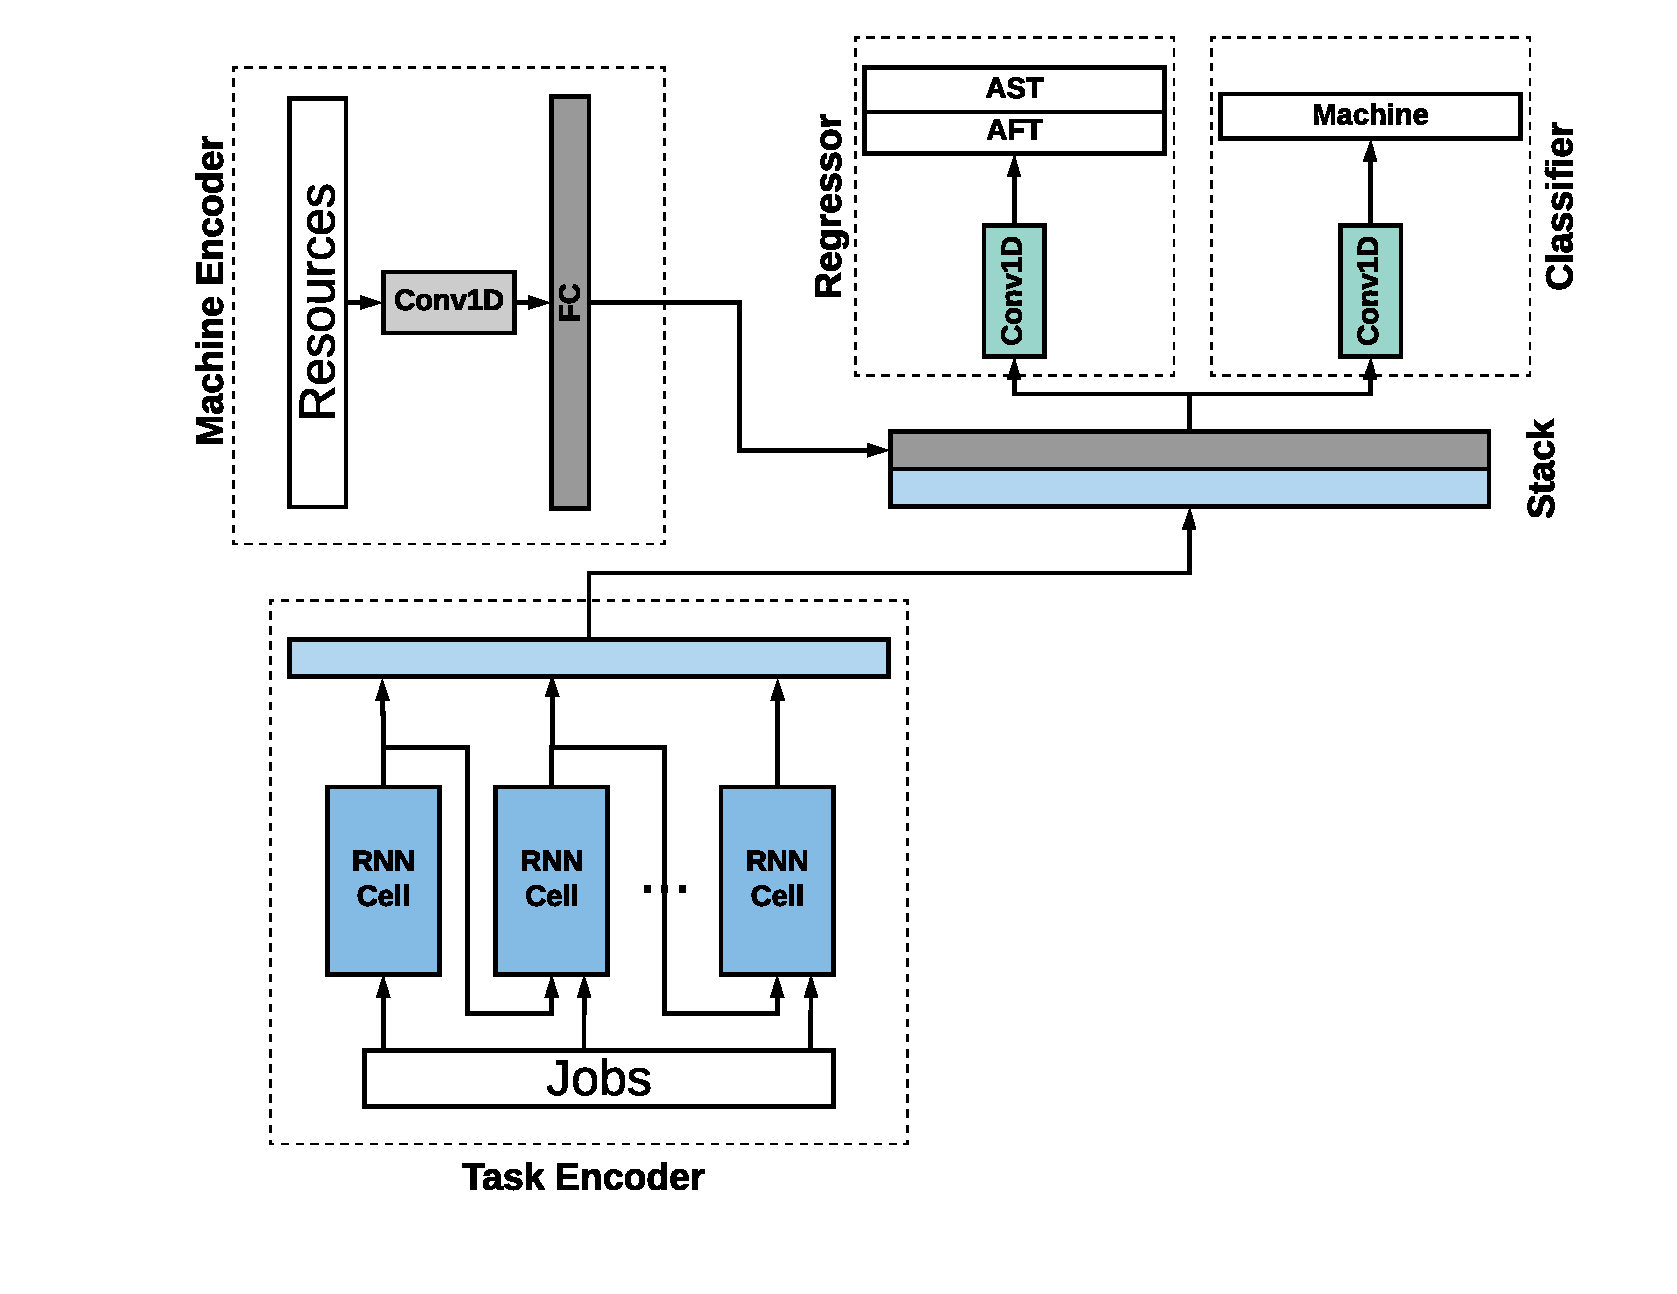
\includegraphics[width=0.45\textwidth]{sched_nn}
    \caption{The architecture of the proposed neural network for distributed heterogeneous systems scheduling}
    \label{fig:nn}
\end{figure}
    
\subsubsection{Objective Function}
The cost function defined for this architecture is a sum of two criteria. Categorical cross entropy \emph{(CE)} on the predicted machine to run a specific job $M_p$ and mean square error \emph{(MSE)} on the predicted actual start time $AST_p$ and the predicted actual finish time $AFT_p$. So it can be summarized as follows:
\begin{equation}
\mathcal Loss(L) = CE(M_p, M_t) + MSE(AT_p, AT_t)
\end{equation}
where $M_p$ is the predicted machine, $M_t$ is the ground truth machine, $AT_p$ is the predicted actual time range and $AT_t$ is the ground truth actual time range.

\subsubsection{Downsides}
The main downside of the proposed solution is that we have to know the maximum number of machines and the maximum number of tasks to be able to define the network. These numbers are used to define the network and loss function dimensions. 
    
\section{Experimental Setup}

\section{Discussion and Results}

\section{Conclusion}

\medskip

\bibliographystyle{unsrt}
\bibliography{paper}
    
\end{document}
